\section{The proposal}\label{sec:proposal}

As discussed in Section~\ref{sec:problems}, relational databases are
often hard to maintain and share. Also, the idea of having in-house
developed and closed source information systems is being increasingly
replaced by the concept of open source systems. In such systems the
responsibility of updating and creating new features is not sustained
by a single institution but usually by a whole community that share
knowledge and interests with associates. In this way the system is
kept up-to-date, accessible and improving much faster due to the
increased number of contributors. Such systems are usually compatible
with standards so as to ensure they can be widely used.

Our objective is to propose the use of modern tools so CPDOC can
improve the way they maintain, store and share their rich historical
data. The proposal privileges open source systems and a lightweight,
shared way of dealing with data. Concretely, we propose the
substitution of the three CPDOC systems by the following technologies.

% It is important to mention that CPDOC has currently three different
% information systems. Althought in the first stage the pilot project
% will involve only the DHBB system, this article is about the whole
% vision of the CPDOC data migration. This system was chosen due to
% different administrative reasons, but also because it has the
% simplest data model.

The Acessus data model comprises personal archives that contains one
or more series (which can contain also other series in a stratified
hierarchy) of digitalized documents or photos. The PHO system data
model is basically a set of interviews grouped according to some
defined criteria within the context given by funded projects. For
instance, a political event could originate a project which involve
interviewing many important people taking part on the event.

Therefore, Acessus and PHO systems can be basically understood as
systems responsible for maintaining collections of documents organized
in a hierarchical structure. In this way, one can assume that any
digital repository management system (DRMS) have all the required
functionalities. Besides, DRMS usually have desirable features that
are not present in Acessus or PHO, such as: (1) data model based on
standard vocabularies like Dublin Core~\cite{dc} and SKOS~\cite{skos};
(2) long-term data preservation functionalities (tracking and
notifications of changes in files); (3) fine-grained access control
policies; (4) flexible user interface for basic and advanced queries;
(5) compliance with standard protocols for repositories
synchronization and interoperability (e.g., OAI-PMH~\cite{oai}); (6)
import and export functionalities using standard file formats and
protocols; and more.

In our proposal Acessus and PHO systems data and files are planned to
be stored in an open source institutional repository software such as
Dspace~\footnote{\url{http://www.dspace.org/}} or Fedora Commons
Framework~\footnote{\url{http://www.fedora-commons.org}}.
% or a more specialized repository management system like
% ICA-AtoM~\cite{van2009ica}~\footnote{\url{https://www.ica-atom.org}}.
In this article we assume the adoption of Dspace with no prejudice of
theoretical modeling.

% These projects are the motivation and origin of financial support
% for a series of interviews conducted by CPDOC team with a specific
% purpose.

The DHBB relational model can be summarized to a couple of tables that
store metadata about the dictionary entries (stored in a single text
field of a given table). The actual dictionary entries are created and
edited in text editors outside the system and imported to it only
after being created and revised.

% In this way, the system does not maintain the history of
% changes. The content of the entries are saved in HTML~\cite{xhtml}
% format. The HTML is generated by the different text editors used
% making it not uniform, clean or portable and long-term compatible.

The nature of its data suggests that DHBB entries could be easily
maintained as text files using a lightweight human-readable markup
syntax. The files would be organized in an intuitive directory
structure and kept under version control for coordinated and
distributed maintenance. The use of text
files~\footnote{\url{http://en.wikipedia.org/wiki/Text_file}} is
justified by a couple of reasons. They are: easy to maintain using any
text editor (tool independent) allowing the user to use the prefered
text editor; conform to long-term standards by being software and
platform independent; easy to be kept under version control by any
modern version control
system~\footnote{\url{https://en.wikipedia.org/wiki/Revision_control}.}
since they are comparable (line by line); and efficient to store
information~\footnote{A text file of a DHBB entry has usually 20\% the
  size of a file DOCX (Microsoft Word) for the same entry.}.

The use of a version control system will improve the current workflow
of DHBB reviewers and coordinators, since presently there is no aid
system for this task, basically performed using Microsoft Word text
files and emails. The adoption of such tool will allow file exchanges
to be recorded and the process controlled without the need of
sophisticated workflow systems, following the methodology developed by
open sources communities for open source software maintenance. For
instance, Git~\footnote{\url{http://git-scm.com}.} is specially suited
to ensure data consistency and keeps track of changes, authorship and
provenance.

% Most of the suggested technologies are of daily use to most people
% with technical profile, such as software developers, but not very
% familiar to people with non-technical profile. In this context, a
% big challenge of this approach is to motivate the internal users of
% CPDOC systems, i.e., CPDOC archives maintainers, to invest their
% time to learn new technologies, instead of keeping their inefficient
% but known way of dealing with data.

Many of the ideas here proposed were already implemented as a proof of
concept to evaluate the viability of such environment in
CPDOC. Figure~\ref{fig:dia-1} illustrates the necessary steps to fully
implement our proposal. In the following text we briefly describe each
step.

\begin{figure}[htbp]
  \centering
  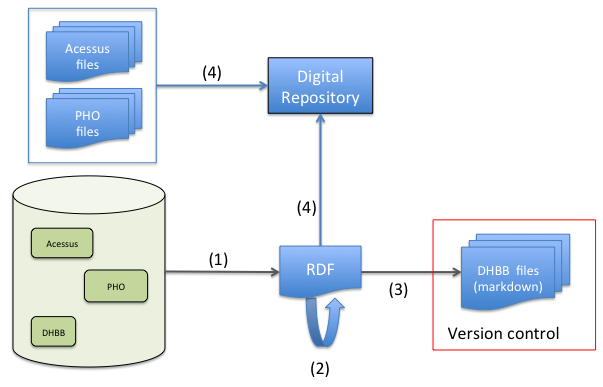
\includegraphics[width=.6\textwidth]{migration.png}
  \caption{Migrating from relational databases to the proposed model}\label{fig:dia-1}
\end{figure}

Step (1) is implemented and the relational database was exported to
RDF~\cite{rdf-primer} using the open source D2RQ~\cite{d2rq} tool. The
D2RQ mapping language~\cite{d2rq-map} allows the definition of a
detailed mapping from the current relational model to a graph model
based on RDF. The mapping from the relational model to RDF model was
already defined using the standard translation from relational to RDF
model sketched out in \cite{dbANDrdf}. The mapping created so far
defers any model improvement to step (2) described below.

% Until CPDOC team decide about the adoption of the proposed
% technologies and for the abandonment of the current architecture,
% the generated RDF can be updated whenever necessary using D2RQ.

Step (2) is planned and represents a refinement of the graph data
model produced in step (1). The idea is to produce a data model based
on standard vocabularies like Dublin Core~\cite{dc}, SKOS~\cite{skos},
PROV~\cite{prov} and FOAF~\cite{foaf}. The use of standard
vocabularies will make the data interchangeable with other models and
facilitate its adoption by service provides and users. It will also
help us to better understand the database model and its semantics. In
Section~\ref{sec:model} we describe the refinement proposal in detail.

Step (3) is already implemented and deploys a text file for each DHBB
entry. Each text file holds the entry text and metadata~\footnote{It
  is out of this article scope to present the final format of these
  files.}.  The files use YAML~\cite{yaml} and
Markdown~\cite{markdown} markup languages to describe the metadata and
entry content. YAML and Markdown were adopted mainly because both
languages are human-readable markups for text files and are supported
by almost all static site generators~\footnote{In this application we
  used Jekyll, \url{http://jekyllrb.com}, but any other static site
  generator could be used.}. The use of a static site generator allows
DHBB maintainers to have full control over the deployment of a DHBB
browsable version.

% Using some scripts that we can easly develop they could deploy a
% DHBB version in three steps: (a) syncronized his repository with the
% repository of other contributors; (b) check the text files to make
% sure that the necessary metadata are presented and have the expected
% values; and (c) compile the files generating a complete website that
% could be made available for the public using a web server and even
% distributed in mirrors servers.

% Actually, each DHBB contributor could generate his one browsable
% DHBB for navigate through the DHBB entries.

Note that step (3) was actually implemented to use the initial version
of the RDF produced in step (1). The code can be easily adapted to use
the final RDF model produced by step (2).

In the planned step (4) the digital files and their metadata will be
imported into a DRMS. This step is much more easily implemented using
the RDF produced in step (2) than having to access the original
database. It is only necessary to decide which repository management
system will be adopted.
% , install it in a server and create the necessary scripts.

% Considering that all DRMS have detailed control access mecanisms, we
% believe that both high and low resolution files can be imported to
% the same digital repository making only the low resolution open for
% public access. This is necessary mainly for preserve bandwidth and
% because in general, the low resolution files also contain some
% watermark and embeded metadadata.

% The migration of the data from relational databases to
% RDF~\cite{rdf} and a simple prototype for browse the data was
% implemented using Jekyll System~\footnote{\url{http://jekyllrb.com}}
% and query support was provided by Apache Solr~\cite{solr} was built
% and used.

The proposed workflow architecture is presented in
Figure~\ref{fig:dia-2}.
% and will be described briefly in what follows. Remember that
Recall that one of the main goals is to make CPDOC archive collections
available as open linked data. This can be accomplished by providing
data as RDF/OWL files for download and a SPARQL Endpoint~\cite{sparql}
for queries. Since data evolve constantly, CPDOC teams would deliver
periodical data releases. Besides the RDF/OWL files and the SPARQL
Endpoint, we believe that it is also important to provide a
lightweight and flexible web interface for final users to browse and
query data. This can be easily done using a static website generator
and Apache Solr~\footnote{\url{http://lucene.apache.org/solr/}} for
advanced queries. As a modern index solution, Solr can provide much
powerful and fast queries support when compared to traditional
relational database systems. Note that the produced website, the
RDF/OWL files and SPARQL Endpoints are complementary outputs and serve
to different purpose and users.
% This sum up the ideas of the architecture.

\begin{figure}[htbp]
  \centering
  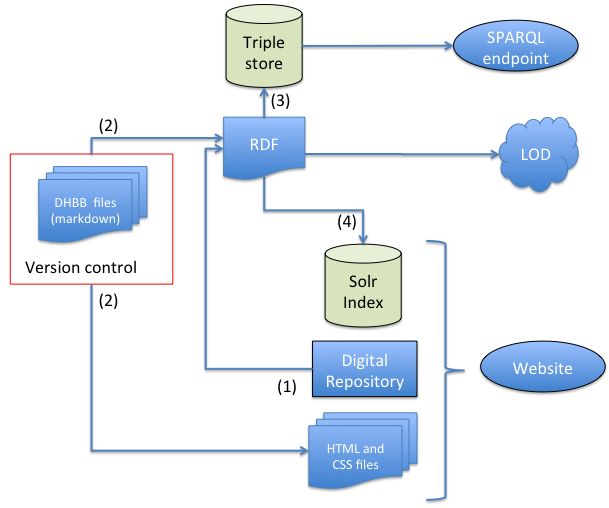
\includegraphics[width=.6\textwidth]{new-architecture.png}
  \caption{The final architecture}\label{fig:dia-2}
\end{figure}

Finally, it is vital to stress the main contrast between the new
architecture and the current one. In the current CPDOC architecture
the data is stored in relational databases and maintained by
information systems. This means that any data modification or
insertion is available in real time for CPDOC website users. However,
this architecture has a lot of drawbacks as mentioned in
Section~\ref{sec:problems}, and also the nature of CPDOC data does not
require continuous updates, which means that the cost of this
synchronous \emph{modus operandi} is not needed. Usually, CPDOC teams
work on projects basis and therefore new collections, documents and
metadata revisions are not very often released.

% \section{DHBB: study of case}

% The scope of the proposed implementation is limited, at first, to
% the entries of DHBB. The reason lies in the fact that the data model
% is the simplest of the three and also due to the unconditional
% support received by DHBB managers for our reformulation.  We aim to
% implement a lightweight web interface prototype for browsing and
% querying CPDOC's collections; scripts to produce the RDF file for
% distribution of CPDOC archives releases; scripts to upload the CPDOC
% collections and files into the Dspace system; and a git repository
% for the DHBB files. All these steps are described in this section.

% illustrates the steps of the migration process from the relational
% database to the proposed model. In step (1) the relational database is
% exported to an RDF file using the open source D2RQ~\cite{d2rq}
% tool. The D2RQ mapping language~\cite{d2rq-map} allows the definition
% of a detailed mapping from the current relational model to a graph
% model and implements most of the ideas currently recommended by the
% W3C's R2RML mapping language~\cite{r2rml}.

% The Acessus and PHO collections of documents, images, audio and video
% files will be stored in the DRMS. Users can consult the DRMS directly
% or the collections and items metadata could be exported and integrated
% with additional information (DHBB and complementary data) into the
% final model (one or more RDF files). DHBB editors could generate from
% the YAML+Markdown some RDF files.

% In step (1) a script is used to syncronize the triple store with the
% digital repository metadatas. In step (2) the DHBB files are processed
% to generate the static website... the PHO and Acessus digital
% repository is queried and a RDF file is produced with a dump of its
% current state. The RDF files generated in steps (1) and (2) are
% combined into a single RDF file that is imported to a triple store. In
% (3) the combined RDF file with a snapshot of CPDOC data is made
% available for download or queries through a SPARQL Endpoint provided
% by the Triple Store. In (4) a Solr Instance Index is updated, serving
% as a back-end to a lightweight web interface that provides faced
% search and browsing interfaces of an integrated view of CPDOC
% collections. As a modern web development framework, Solr can provide
% much better and fast queries support when compared to traditional
% relational database systems.

% It is possible to notice that the steps of Figure~\ref{fig:dia-2}
% need not be synchronized, even though CPDOC teams could agree to
% follow a common data release schedule. For instance, if a specific
% release of CPDOC complete archives is planned but the DHBB team was
% not able deliver a new DHBB version in time, new RDF/OWL files
% release can be delivered normally. It would contain the last
% versions delivered by each team, with no prejudice to the others.

The results obtained so far encouraged us to propose a complete data
model aligned with open linked data vocabularies, presented in detail
in next section.

% FICOU MUITO FORA DE CONTEXTO To make CPDOC data widely used and
% available, we also suggest that CPDOC should define a annual
% schedule for distribution snapshots of its archives in RDF
% format. The RDF file(s) could be offer for download and online
% available for queries in a triple store with a SPARQL endpoint. In
% the next section we further describe the proposal architecture.

% In step (2) scripts use the RDF file produced in the step (1) to
% migrate files and metadata of Acessus and PHO systems to the open
% source repository software DSpace. The mapping of Acessus data to
% Dspace is described in Table~\ref{tab:map}. The mapping of PHO
% interviews is basically consisted of linking each project to a
% collection and each interview to an item with the respectively
% bitstreams (digital audio or video files).

% \begin{table}[htbp]
% \centering
% \begin{tabular}{rcl}
% Acessus &  & Dspace \\ \hline
% personal archives & $\to$ & communities \\
% series & $\to$ & collections \\
% documents or photographies metadata & $\to$ & items \\ 
% documents or photographies files & $\to$ & bitstreams \\ \hline
% \end{tabular}
% \caption{Mapping from Acessus to Dspace}\label{tab:map}
% \end{table}

% In step (3) the RDF model created is improved based on linked data
% concepts, i.e., considering the adoption of standard vocabularies and
% ontologies such as FOAF~\cite{foaf}, SKOS~\cite{skos}, Dublin
% Core~\cite{dc} and PROV~\cite{prov}. This refined RDF file would be
% available in form of periodic releases of CPDOC's collections that
% would be much more interoperable and useful for service providers.

% In step (4) Markdown~\cite{markdown} files are created using
% YAML~\cite{yaml} metadata header for each DHBB entry. YAML is a
% lightweight markup language for metadata description in a
% human-readable text file, while Markdown allows people to write text
% using an easy-to-read, easy-to-write plain text format that can be
% converted to structurally valid XHTML~\cite{xhtml} (for online use) or
% PDF (for printing). These files can be host in a distributed
% versioning control environment for collaborative maintenance. This can
% be achieved using Git~\cite{git}, a distributed version control system
% which is suitable for many different models of collaborations.

% Some tools are available for this kind of conversion and one of the
% most established is the D2RQ~\cite{d2rq}. Once the RDF is generated,
% several steps for improving and enriching the RDF file, checking for
% data consistency and gathering new data connections using the
% available knowledge sources (ontologies, dictionaries etc) is
% planned.  This environment of a group of files organized in a
% directory structure under control of a version control system and
% the RDF interface is meant to compose the new data storage for DHBB.

% Figure~\ref{fig:dhbb-ex} shows a fragment of a YAML+Mardown file from
% a DHBB entry, just as an example. Lines 1--16 are the YAML header with
% the metadata about the entry. The entry content is written in Markdown
% as observed from the line 17 on. In Line 18 it is possible to see that
% references to metadata fields can be made inside the body of the entry
% written in Markdown.

% \begin{figure}[thbp]
%   \centering
% \begin{lstlisting}[frame=single,numbers=left,basicstyle=\footnotesize\ttfamily]
% ---
% type: biliography
% created-by: 2010-03-04T17:55:58,83Z
% title: Assad Junir, Mario
% reviewer: Fulano
% author: Beltrano
% positions: 
%  - dep. fed. MG 1998-1999
%  - dep. fed. MG 2000-2002
%  - dep. fed. MG 2003-2007
% sources: 
%  - Camara dos Deputados; DIAP (Ago./06); Diario de Sao Paulo
%    (online) 29/10/2003. at http://oglobo.globo.com/diariosp.
%  - Portal Caparao (online) 01/jun/2007 e 15/maio/2008. Disp.
%    em http://www.portalcaparao.com.br.
% ---

% {{ title }}

% *Mario Assad Junior* nasceu em Manhuacu (MG) no dia 11 de 
% agosto de 1965, filho de [Mario Assad](/dhbb/mario-assad.html) 
% e de Nedi Vieira Assad. Seu pai foi deputado estadual em Minas 
% Gerais de 1967 a 1975 e de 1978 a 1983, secretario do Trabalho, 
% Acao Social  e Desporto de 1975 a 1978, deputado federal de 
% 1983 a 1991, secretario de Justica de 1991 a 1994 e prefeito 
% de Manhuacu entre 2001 e 2004.
% ...
% \end{lstlisting}
% \caption{YAML+Markdown file of a DHBB entry}\label{fig:dhbb-ex}
% \end{figure}

% Figure~\ref{fig:dia-2} shows how the CPDOC data is supposed to be
% maintained in our model. In step (1) a script is used to generate the
% current DHBB repositoty state RDF file for a DHBB maintainer. In step
% (2) the PHO and Acessus digital repository is queried and a RDF file
% is produced with a dump of its current state. The RDF files generated
% in steps (1) and (2) are combined into a single RDF file that is
% imported to a triple store. In (3) the combined RDF file with a
% snapshot of CPDOC data is made available for download or queries
% through a SPARQL Endpoint provided by the Triple Store. In (4) a Solr
% Instance Index is updated, serving as a back-end to a lightweight web
% interface that provides faced search and browsing interfaces of an
% integrated view of CPDOC collections. As a modern web development
% framework, Solr can provide much better and fast queries support when
% compared to traditional relational database systems.

% \begin{figure}[thbp]
%   \centering
%   \includegraphics[width=.9\textwidth]{diagrama2.png}
%   \caption{Data maintainance}\label{fig:dia-2}
% \end{figure}

% It is possible to notice that steps (1) and (2) of
% Figure~\ref{fig:dia-2} need not be synchronized, even though CPDOC
% teams could agree to follow a common data release schedule. For
% instance, if a specific release of CPDOC complete archives is planned
% but the DHBB team was not able deliver their version in time, the
% release can be delivered normally. It would contain the last versions
% delivered by each team, with no prejudice to the others.

%%% Local Variables: 
%%% mode: latex
%%% TeX-master: "article"
%%% End: 
